\documentclass[12pt]{article}
\usepackage{fancyhdr}
\usepackage{datetime}
\usepackage{graphicx}
\usepackage{amsmath}
\usepackage{float}
%\usepackage{showframe}

%custom variables
\newdate{date}{16}{09}{2016}
\newcommand{\hwNum}{1}
\newcommand{\type}{Lab No.}
\graphicspath{ {images/} }


%header
\pagestyle{fancy}
\lhead{Daniel Andronov}
\chead{\thepage}
\rhead{\type{} \hwNum{}}
\cfoot{\thepage}

\fancyheadoffset[LO,RE]{1pt}
\fancyheadoffset[RO,LE]{1pt}

%titlepage
\title{\type{} \hwNum{}}
\author{Daniel Andronov}
\date{\displaydate{date}}

%addition settings
\topmargin=-0.45in
\evensidemargin=0in
\oddsidemargin=0in
\textwidth=6.5in
\textheight=9.0in
\headsep=0.25in

\begin{document}
\maketitle
\newpage

\section{Questions from Seciont 2.3}


\paragraph{Problem 1}
During the first iteration, the total load, $L$ on node 0 is \\
\begin{align}
 L & = \frac{ R_{agg} }{Link Cap }  = \frac{  4 \times R_a }{1 Mb/s }\\
&   = \frac{ 4\times R_p \times F_{on} }{1 Mb/s } = \frac{500 Kb/s}{1Mb/s} = 0.5 
\end{align}
So, the total load on node 0 is 0.5. However, it is still possible to incurr packet loss if all nodes transmit at once, which has a probability of $1/2^4$ or 6.25\% chance of occuring. 

\paragraph{Problem 2}
I first observed packet loss occuring during the third iteration when the load on node0 was 60\%. Even though the load is much less than one, if all nodes transmit at once then the node will have to deal with traffic incoming at 1.2Mb/s, which is over the link capacity. 

\paragraph{Problem 3 \& 5}
The figure below illustrates the relationship between the load on node 0, packet loss, and average packet delay. 
\begin{figure}[H]
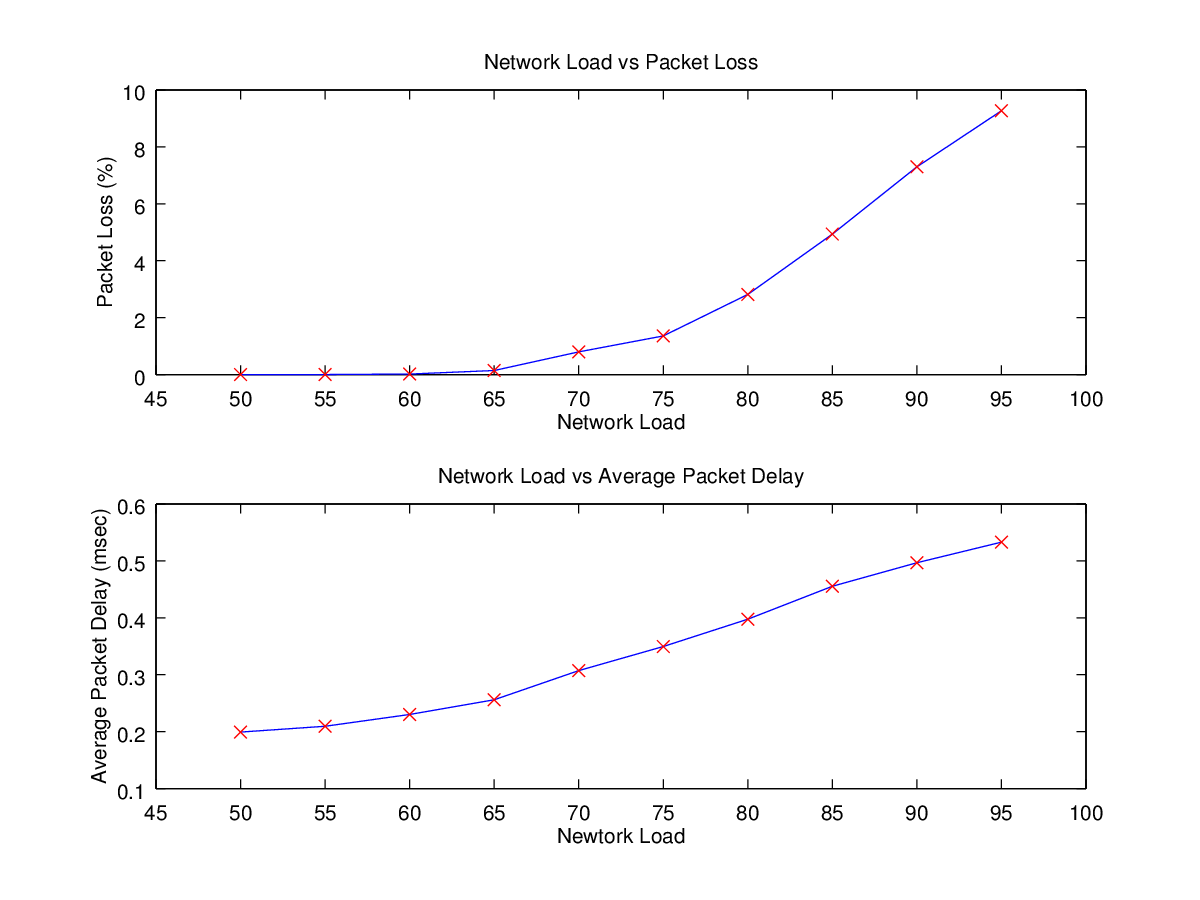
\includegraphics[ width=\textwidth, scale = 0.05 ]{fig}
\end{figure}

\paragraph{Problem 4}
The minimum and maxium intervals are detailed in following table. Let $R_pi  = 250 + 25i$, where $i\in {0, 1, ..., 9, 10}$, be the peak rate of each node per iteration i. The minimum delay per pracket would be the time to get the packet on the link, then propagating through two links. Thus, \\
$$t_{min} = t_{xmit} + 2t_{prop} = 0.02 + \frac{ 8,000 }{ 250 + 25i } ms$$.

The maximum delay time would include the minimum delay time but also have to account for the packet arriving just as a full buffer has release a packet so that the buffer would be filled again. This the packet being tracked will have to wait for 9 packets to clear the queue before it itself could be put on the link. Thus, \\
\begin{align}
t_{max} & = t_{min} + 10\frac{ 80 }{ 250 + 25i Kb/s }\\
& = 0.02 + \frac{ 8,000 }{ 250 + 25i } + \frac{ 80,000 }{ 250 + 25i } \\
& = 0.02 + \frac{ 88,000 }{ 250 + 25i } ms\\
\end{align}
Using these equations, the table below was generated. 

\begin{center}
	\begin{tabular}{ | l | l | l | }
	\hline
	Iteration & Min Delay (ms) & Max Delay (ms)\\ \hline
	0 & 32.02 & 352.02 \\ \hline                                                                                             
	1 & 29.02 & 320.02 \\ \hline                                                                                             
	2 & 26.02 & 293.02 \\ \hline                                                                                             
	3 & 24.02 & 270.02 \\ \hline                                                                                             
	4 & 22.02 & 251.02 \\ \hline                                                                                             
	5 & 21.02 & 234.02 \\ \hline                                                                                             
	6 & 20.02 & 220.02 \\ \hline                                                                                             
	7 & 18.02 & 207.02 \\ \hline                                                                                             
	8 & 17.02 & 195.02 \\ \hline                                                                                             
	9 & 16.02 & 185.02 \\ \hline
	\end{tabular}
\end{center}

\end{document}
This is never printed